\subsection{JIT Architecture}

The JIT emulator functions by partitioning the program, as it is executed, into source blocks. These blocks are compiled into corresponding x86 host blocks. Each host block terminates by returning an address, corresponding to the exiting MIPS program counter (PC). For blocks without a terminating jump, this will be the subsequent instruction. The system will then execute the block at the desired PC, compiling a new host block if required.

\begin{figure}[h]
    \centering
    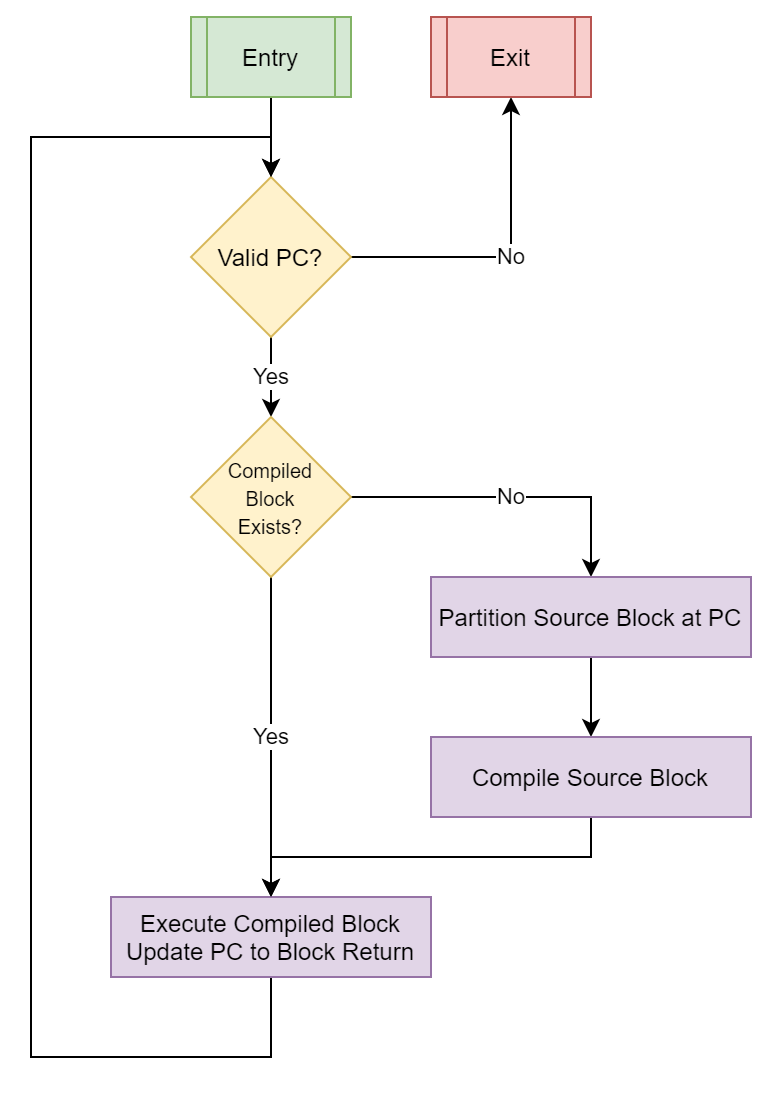
\includegraphics[width=0.5\linewidth]{diagrams/jit.png}
    \caption{Top level architecture of the JIT emulator.}
    \label{figure:jit-arch}
\end{figure}

This architecture was chosen as compiled host blocks cannot have a jump compiled directly to the desired PC, as the destination may not be compiled yet. Further work will investigate retroactively patching a direct jump into the compiled host blocks when possible to improve performance.

\subsubsection{Runtime}

The runtime is the top level JIT emulation system and ties together all the other JIT components. When provided with a MIPS program the runtime will then emulate it by partitioning it into blocks and compiling them with the compiler. The current implementation terminates a source block when a jump instruction is encountered, but other partitioning schemes will be investigated. These compiled host blocks are stored in a cache and re-used on subsequent executions.

\subsubsection{Compiler}

The compiler is used to convert source MIPS blocks into host x86 blocks.

\subsubsection{Assembler}

The assembler is responsible for encoding the desired \texttt{x86} instructions into an internal buffer, which can then be copied into the executable memory buffer once compilation of a block is complete. It makes heavy usage of templates and \texttt{constexpr} evaluation to offload as much work as possible to \texttt{C++} compile time, increasing the runtime performance. It is currently designed to support 8 bit, 16 bit and 32 bit \texttt{x86} instructions.

\subsubsection{Register File}

The register file provides the runtime and compiler with a means of emulating the MIPS register file. The current implementation uses an in memory model, where a C++ array represents the MIPS register bank. Translated x86 instructions load and store this array when they need to emulate a MIPS register modification. The special \texttt{hi} and \texttt{lo} registers in MIPS are mapped internal to \texttt{\$32} and \texttt{\$33} respectively so the same compilation architecture can be used. This memory model provides for fast compile times but subpar execution times, as the contents must be written back after every instruction, causing in some cases large overhead. Other solutions will be explored such as direct register mapping or a hybrid model \cite{mark-probst-dbt}; these should yield increase execution performance, but potentially at the cost of worse compiler performance.

The compiler omits any instructions that would cause a write to \texttt{\$0}, preserving its constant zero value.

\subsubsection{Memory Map}

The memory map uses an associative model powered by an unordered hash table. This allows for the entire 32-bit address space to be emulated without requiring it to be pre-allocated, something that might prove difficult in a 32 bit process. The current implementation allows for \texttt{O(1)} read and write times. Despite this, the performance is substandard compared to a raw array due to the extra overhead and being less cache friendly; further work will explore a hybrid model to utilise additional data structures to accelerate portions of the memory space.

After profiling, the \texttt{std::unordered\_map} originally used was found to be a bottleneck and thus was replaced with a 3rd party implementation Tessil/robin-map \cite{tessil-map, tessil-benchmark}.
